\documentclass[a4paper,12pt]{report}
\usepackage[utf8]{inputenc}
\usepackage[T1]{fontenc}
\usepackage{lmodern}
\usepackage{mathtools}
\usepackage[catalan]{babel}
\usepackage{hyperref}
\usepackage{graphicx}
\usepackage{acronym}
\usepackage{eurosym}
\usepackage{pgfplots}
\usepackage[backend=biber]{biblatex}
\usepackage[auth-sc]{authblk}
\usepackage{siunitx}

\sisetup{round-precision=2,round-mode=figures,scientific-notation=true}

\addbibresource{biblio/main.bib}

\date{}
\begin{document}

\acrodef{ia}[IA]{{inteligència artificial}}
\acrodef{ann}[ANN]{{xarxa neuronal artificial}}


\title{
	{\bf Filosofia del Software\\ i \\Intel·ligència Artificial} \\
}
\author{
	Oriol Ventosa \and
	Marc Ferré \and
	Gonzalo Palacios \and
	Pol Gómez
}

\maketitle

\tableofcontents

\part{Conceptes}


\part{Procediments}

\chapter{Introducció}
Els procediments del projecte de recerca es basen en la realització de diferents \emph{demos} (demostracions)
que tenen la intenció de oferir una introducció a les aplicacions de la \ac{ia}.

S'ha utilitzat el llenguatge de programació C++, i les llibreríes SFML \autocite{sfmllib} (per a gràfics) i FANN \cite{fannlib} (per a la
creació i entrenament de xarxes neuronals).

Les demos (junt amb el seu estat de progrés actual) són les següents:

\begin{itemize}
\item \emph{Demo 1} - joc de futbol sala (5 jugadors per equip), aprenentatje 'per esforç' (reinforcement) amb \ac{ann} evolutiva, estat inicial
\item \emph{Demo 2} - reconeixement de caràcters 0-9, \ac{ann}, estat avançat (ajustament de paràmetres d'aprenentatge, etc)
\item \emph{Demo 3} - conducció automàtica (circuit simple), reinforcement amb \ac{ann} evolutiva, estat inicial (físiques de conducció)
\item \emph{Demo 4} - ?
\end{itemize}

\emph{* La llista de demostracions pot variar fins a la versió final *}


\chapter{Xarxes Neuronals Artificials}
Les \emph{xarxes neuronals artificials} (ANN) són \emph{models computacionals 
inspirats pel sistema nerviós central dels animals (en particular, el cervell)} \autocite{nnpatrec}.

L'estructura d'una \ac{ann} és semblant a la d'un circuit electrònic: hi ha una capa o \emph{layer}
de $ q $ neurones d'entrada, o \emph{inputs}, i un layer de $ p $ neurones de sortida, o \emph{outputs}.
Això permet representar la seva estructura com si fos una funció matemàtica, $ f(x_0, x_1, ..., x_q) = \{y_0, y_1, ..., y_p\} $,
és a dir: un conjunt $ x $ d'entrades formen un conjunt $ y $ de sortides \ref{simple_ann}.

\begin{figure}[ht!]
\centering
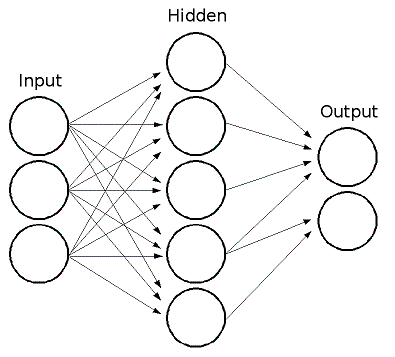
\includegraphics[width=80mm]{data/nn_simple.png}
\caption{El propòsit del layer \emph{hidden} s'explicarà més endavant.}
\label{simple_ann}
\end{figure}

La tasca principal d'una xarxa neuronal \emph{supervisada} és realitzar una \emph{aproximació de funció},
és a dir, a partir d'un seguit de valors de la funció (anomenat \emph{training set}), $ f(a) = b $, crear un model que s'ajusti a les dades
que se li ha subministrat \ref{func_approx}. Podríem, per exemple, entrenar una \ac{ann} per a que realitzés
una aproximació de la funció $ sin(x)$, però és més interessant entrenar-la amb objectius més sofisticats; tot
problema determinista que es pugui reduir a \emph{produir unes sortides a partir d'uns valors d'entrada}, es pot
solucionar, molt probablement, amb una xarxa neuronal.

\begin{itemize}
\item \emph{Conduir un cotxe:} la posició, la velocitat, els cotxes adjacents, la carretera... una gran quantitat d'entrades. La nova direcció, 
accelerar o frenar, com a sortides.
\item \emph{Predir el flux del mercat de valors:} la pendent de la gràfica del valor d'una acció, els últims moviments, els últims compradors...
la xarxa s'ha entrenat amb dades històriques, i l'historia es repeteix. El moviment de l'accionista com a sortida.
\item \emph{Reconèixer caràcters:} aquesta és la nostra parada per a continuar amb l'explicació de les \ac{ann}. El conjunt de píxels que formen 
l'imatge d'un caràcter com a entrades, i el número que representen els píxels com a sortida. És un exemple fàcil d'aplicar i enriquidor.
\end{itemize}

\begin{figure}[ht!]
\centering
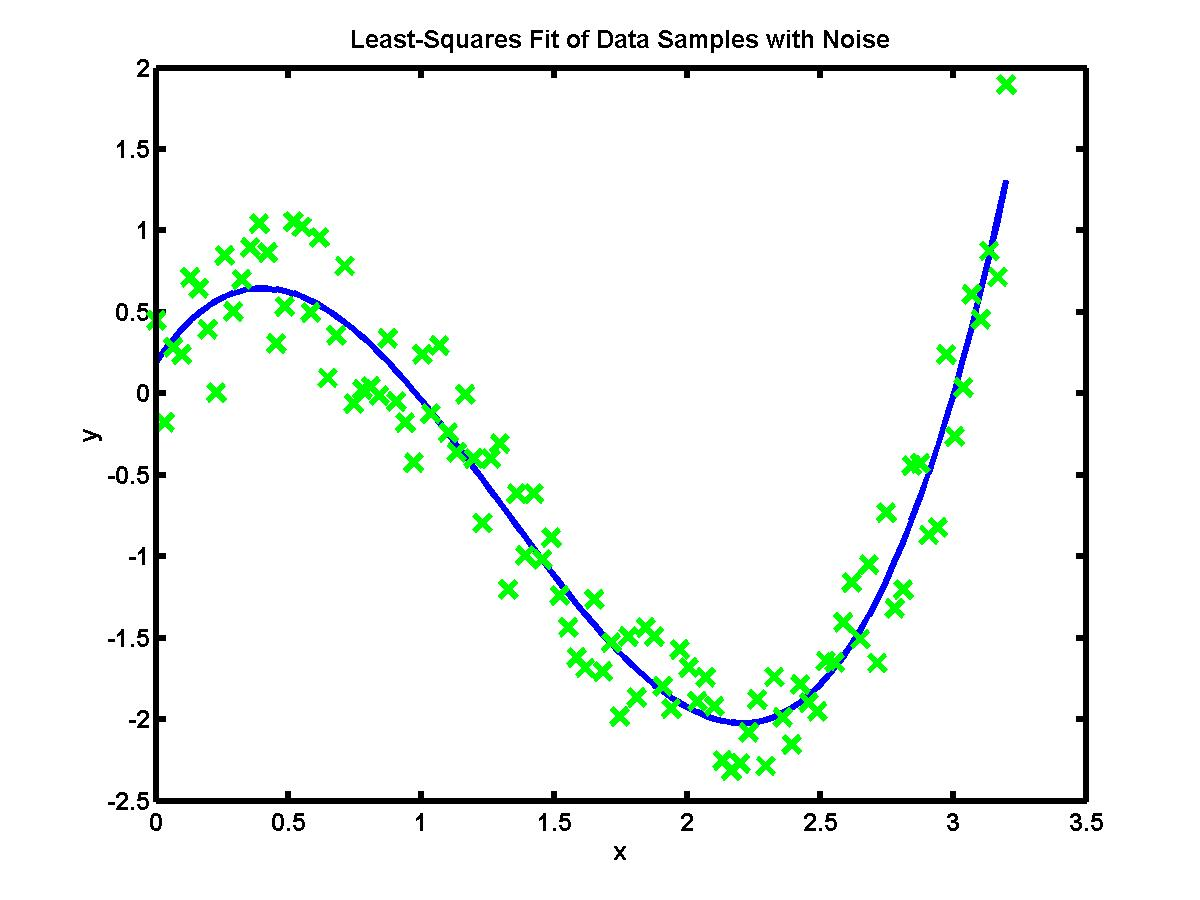
\includegraphics[width=80mm]{data/func_approx.jpg}
\caption{Exemple d'aproximació de funció. Els punts verds són els valors subministrats, el training set,
i la línia blava la funció que s'ha aproximat.}
\label{func_approx}
\end{figure}

\chapter{Reconeixement de Caràcters}
\begin{figure}[ht!]
\centering
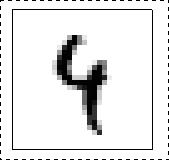
\includegraphics[width=35mm]{data/confusing_2.png}
\caption{4 o 9? La nostra \ac{ann} creu amb un 100\% de certesa que és un 4, i amb un 47\% de certesa que és un 9.}
\label{certesa}
\end{figure}

Podem visualitzar perfectament el model neuronal que representa un problema de reconeixement de caràcters: la nostra
base de dades, o \emph{dataset}, consisteix de 1000 formes d'escriure cada número, del 0 al 9. És a dir, la xarxa neuronal
no aprendrà només com en Xavi dibuixa el 5, sinó que aprendrà també com el dibuixen 999 persones diferents, exposició suficient per
a poder realitzar una extracció de característiques, o \emph{feature extraction}.

Això és vital, extreure característiques, i per aconseguir-ho necessitem utilitzar un layer addicional, el \emph{hidden}. 
Si realitzéssim l'entrenament amb un layer d'inputs i un layer d'outputs, la interpolació que es produiria seria lineal,
es a dir, es realitzaria un motlle amb el qual es compararia qualsevol imatge, i la major part d'elles no entrarien dins
els paràmetres del motlle (la \emph{dimensionalitat} és única). El que volem es que la xarxa neuronal descobreixi que el número
vuit hauria de tenir dos cercles, que el set és com un 1, però amb un vèrtex desplaçat, que el quatre pot ser un triangle o un
quadrat obert per amunt, ... imagines haver de programar totes aquestes condicions de forma manual? Si no t'ho pots imaginar, 
et deixem la resposta: és un suïcidi.

La xarxa neuronal utilitza el layer hidden per a fabricar un \emph{motlle flexible} i sofisticat, que reconeix certes característiques
en comptes de forçar un model universal. Aquí és quan les \ac{ann}s brillen per complet; són capaces de crear una \emph{caixa negra}
extremadament interconnectada i intel·ligent, que sembla utilitzar raonament, evidentment, intel·ligent. En realitat no hi ha màgia, 
és tot producte d'un magnífic i complex model matemàtic.

\begin{figure}[ht!]
\centering
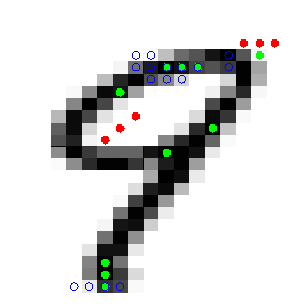
\includegraphics[width=45mm]{data/extraction-0.png}
\caption{Exemple d'extracció de característiques. Gràcies a \href{http://clopinet.com/isabelle/Projects/ETH/}{Isabelle Guyon} \autocite{guyonfe}.}
\label{extracció}
\end{figure}

Nosaltres hem extret un dataset \href{http://cis.jhu.edu/~sachin/digit/digit.html}{derivat} del majestuós \href{http://yann.lecun.com/exdb/mnist/}{MINST} (derivat al seu torn del NIST)
que ofereix deu arxius binaris amb 28x28 píxels per imatge, 1 byte per píxel. El procés que hem seguit per a produir una demostració efectiva de les 
xarxes neuronals en reconeixement de caràcters ha estat el següent:

\begin{enumerate}
\item Establint un índex d'arxiu (del 0 al 9) i un índex d'imatge (del 0 al 999), carreguem l'arxiu adient a l'índex i l'emmagatzemem en un gran vector. A través del teclat, podem
navegar les diferents imatges de cada nombre. Es carrega llavors l'imatge en un panell, per a poder-ho visualitzar.
\item Prement la tecla \emph{C} (de \emph{convert}), el programa crea un arxiu adequat al format que utilitza la llibreria de \ac{ann}s. Importa i normalitza una certa quantitat 
de mostres en un sol arxiu, perfecte per a entrenar la \ac{ann}.
\item Prement la tecla \emph{L} (de \emph{learn}, aprendre), el programa crea una \ac{ann} amb 784 neurones d'entrada, 392 neurones hidden, i 10 neurones de sortida: 3 milions de connexions. Utilitza la 
llibreria per a llegir l'arxiu convertit anteriorment, i entrena la \ac{ann} amb un mètode popular anomenat \emph{backpropagation}. Consisteix en establir uns pesos aleatoris 
en totes les neurones, a l'inici del programa. Llavors, donat un set d'entrenament, prova a calcular el resultat de la xarxa amb unes certes entrades del set, i el compara amb el resultat
que hauria d'obtindre. A través de l'error obtingut, realitza una marxa enredera recursiva, i ajusta els pesos de les neurones de forma que produeixin outputs similars a la que
estableix el set d'entrenament. Realitza tot aquest procés per cada imatge de les 7500 que li deixem per a entrenar.
\item Prement la tecla \emph{T} (de \emph{test}, comprovar), el programa utilitza l'índex corresponent a l'imatge que l'usuari està veient en pantalla, i estableix els seus píxels
com a entrades d'una \ac{ann} creada a partir de l'entrenament anterior. Produeix llavors, la desitjada sortida que estàvem esperant, imprimint a la consola (l'objectiu és dibuixar un gràfic)
la certesa per cada número de l'1 al 9.
\end{enumerate}


\begin{figure}[ht!]
\centering
\includegraphics[width=65mm]{data/test.png}
\caption{Sortida de la nostra xarxa neuronal, per a un estrany número 8. En molts casos, els números 5, 6 i 8 comparteixen característiques. La xarxa neuronal les descobreix.}
\label{output}
\end{figure}



\chapter{Conducció Automàtica}
\begin{figure}[ht!]
\centering
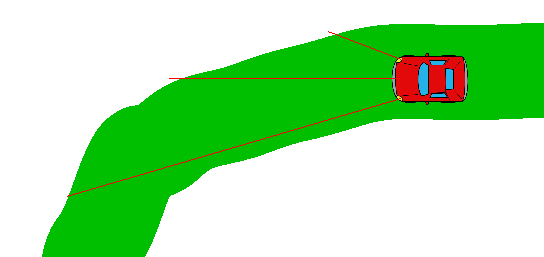
\includegraphics[width=65mm]{data/car1.png}
\caption{Els sensors detecten la distància del cotxe a les parets del circuit.}
\label{sensors}
\end{figure}

La nostra segona demostració és radicalment diferent a la primera:
l'objectiu és programar un automòbil el qual, a partir de tres sensors frontals,
sigui capaç d'evitar xocar amb les parets de \emph{qualsevol circuit}.
És a dir; el seu entrenament ha de ser general i adaptable a qualsevol situació.

Per a solucionar un problema com aquest, no disposem d'un \emph{dataset},
com en el cas del reconeixement de caràcters: qui s'ha dedicat a crear
una base de dades que representa totes les decisions que hauria de prendre
el cotxe, en qualsevol dels casos en que es pot trobar? Evidentment, no és
una tàctica adequada.

Hem d'atacar el problema des d'un altre punt de vista: ara ja no es tracta
d'una situació en la qual l'entrenament de l'agent es pugui supervisar
(\emph{supervised learning}), ara ha d'ésser ell mateix qui explori l'entorn
en el qual es troba. Utilitzarem el segon mètode més popular d'aprenentatge
de màquina: l'aprenentatge sense supervisió (\emph{unsupervised learning}, o \emph{reinforcement learning}).
\\

\section{Reinforcement Learning}

\begin{figure}[ht!]
\centering
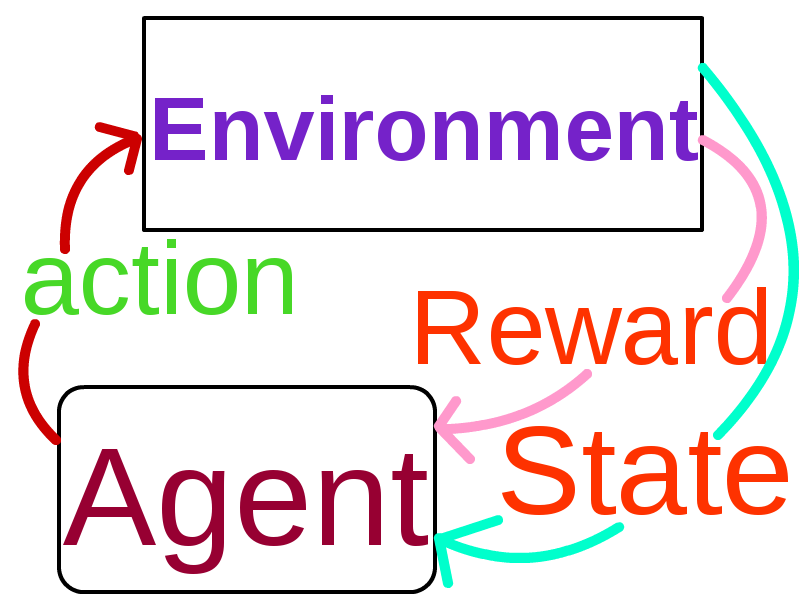
\includegraphics[width=52mm]{data/reinforce.png}
\caption{Diagrama que representa l'aprenentatge per reforç.}
\label{reinforcegraph}
\end{figure}

L'\emph{aprenentatge per reforç} es basa en la presa de decisions de l'agent en base
a una prèvia exploració de l'entorn, la qual ha sigut controlada a través d'un sistema
de recompenses \cite{reinflnbk}.

Ho podem il·lustrar de forma senzilla: un ratolí representa el nostre agent. Aquest divaga
de forma aleatòria a través d'un entorn desconegut. Quan cau en una trampa, se li dona una
recompensa negativa; quan es troba amb un tros de formatge, una de positiva. Poc a poc,
el ratolí aprendrà a evitar trampes i buscar el formatge.

Expressat amb termes més tècnics: el ratolí es troba en un estat \(s\) (que
emmagatzema la quantitat de peces de formatge que té, i si està viu o no), i
realitza una acció \(a\). Això el porta a trobar-se en un estat \(s'\).
Es fa llavors una comparació entre els dos estats, \(s\) i \(s'\), i se
li dona una recompensa \(r\) en base a uns criteris (per cada tros de formatge
que hagi guanyat, \(+5\); si segueix viu, \(+1\); si ha caigut en una trampa,
\(-100\)).

Aquesta és l'essència
de l'aprenentatge per reforç.

\section{Q-Learning}

\emph{Q-learning} és un algoritme d'aprenentatge per esforç. Expressat de forma
matemàtica:

\begin{equation} \label{eq:qlearning}
Q[s, a] = Q[s, a] + \alpha(r + \lambda V(s') - Q[s, a])
\end{equation}

Però que no espanti massa. En realitat, és extremadament fàcil d'implementar (en 
comparació a l'ús d'una \ac{ann}; no hem ni escrit les fórmules adients, degut a la seva
complexitat). Anem pas per pas, seguint el camí que hem fet per a arribar a 
un programa funcional.

Primer de tot, hem de mesurar l'estat en que es troba el nostre agent. Aquesta mesura ha de tenir les dades
que siguin necessàries per a corregir l'agent. Ens interessa, principalment, la distància
a les parets del circuit. Per a fer-ho efectivament, hem projectat tres \emph{làsers} o
sensors, que s'allarguen fins que el color sobre el qual es troben no és el color del circuit.
Un làser va en direcció igual a la del cotxe, i els altres dos es desvien 15 graus per a obtenir
una visió panoràmica de la posició del vehicle \ref{sensors}. Dibuixar les línies que
representen els sensors ha sigut tot un repte en quant a programació i matemàtiques.

Ara ja podem calcular la llargada dels làsers; és això tot el que necessitem per mesurar l'estat
en que es troba el vehicle i donar-li una recompensa. Però, l'algoritme \emph{Q-learning} té una limitació: la seva aplicació
comporta la creació d'un \emph{array} \footnote{També conegut com a \emph{vector}: llista de valors}
que tindrà una quantitat d'entrades igual a \emph{totes les possibles combinacions d'estat}. És a dir,
en el cas dels sensors del cotxe, que poden arribar a tenir un valor de 1,000 (píxels), l'array
tindrà \num{1000000000} entrades (1000 valors possibles per sensor, multiplicat per si mateix tres vegades, la quantitat
de sensors que tenim). No és viable; hem de \emph{discretitzar} una magnitud que, a efectes pràctics, és contínua.

Per tant, volem convertir el valor del sensor a una categoria del 0 al 9, on 0 significa ``molt a prop'', i 9 ``molt lluny'',
per a poder crear un array de dimensions viables (en aquest cas, tenim 10 estats per sensor, per tant, 1000 estats en total).
Com que ens interessa entrenar amb més precisió els casos en que els sensors tenen distàncies molt curtes (el cotxe està a 
prop de la paret), ens agradaria transformar de forma no simètrica els valors dels sensors, és a dir, que un valor real de
250px es transformi a 5, per exemple, i no a 2.5
Primer vam intentar realitzar aquest procés de discretització a partir d'una transformació logarítmica:
\begin{equation}
s_i(D) = \left\lfloor 9 \frac{ln(D)}{ln(1000)} \right\rfloor
\end{equation}
però els valors resultants estaven massa desproporcionats. Vam decidir fer-ho a la força bruta, establint condicions
simples. No és la solució més elegant, però no podem perdre temps amb qüestions trivials.

L'altra qüestió important és la \emph{taula de recompenses}, que defineix com serà recompensat l'agent. En base a què
hauríem d'establir els valors de la taula? L'impuls primitiu és ben simple: recompensa positiva si l'agent segueix viu,
i recompensa negativa si l'agent ha mort. Però això presenta un problema: encara que l'agent s'aproximi perillosament 
a una paret, la recompensa seguirà essent positiva. Així doncs, veiem que hem de basar la recompensa en la distància dels sensors:
com més curta sigui, recompensa més negativa tindrà. Tot i això, introduïm un altre problema: a mesura que l'agent s'aproximi a una
corba, la recompensa es començarà a reduir, i arribarà un moment que es veurà forçat a girar cua. Finalment, hem arribat a una conclusió
no massa intuïtiva: l'agent haurà de rebre recompenses positives (decreixents, però positives) encara que s'apropi a una paret, per a
afavorir l'exploració de l'entorn. Per tant, la \(r\) de l'equació \ref{eq:qlearning} queda definida
com a la ``suma de les recompenses que reben tots els sensors (3)''. Aquí la taula:

\begin{center} \label{tb:rewards}
    \begin{tabular}{| l | l |}
    \hline
    \(S_i\) & \(r\) \\ \hline
    0 & -10 \\ \hline
    1 & -5 \\ \hline
    2 & -1 \\ \hline
    3 & 0 \\ \hline
    4 & 1 \\ \hline
    5 & 2 \\ \hline
    6 & 3 \\ \hline
    7 & 4 \\ \hline
    8 & 5 \\ \hline
    9 & 6 \\ \hline
    \end{tabular}
\end{center}

Ja només queda establir els valors de les constants \(\alpha\) (proporció d'aprenentatge) i \(\lambda\) (factor de descompte), que equivaldran
a \(0.7\) i \(1\) respectivament.

El nostre agent realitza un \emph{tick} \footnote{Cicle} d'aprenentatge cada \(0.5\) segons, i triga al voltant de tres hores a ajustar els
valors de l'array Q per a funcionar amb desimboltura.

Com podríem millorar el funcionament d'aquesta demo? Principalment, de dos formes:

\begin{enumerate}
\item \emph{Selecció genètica}: fer funcionar a un set de \(n\) agents alhora, i guardar els arrays Q que millor hagin progressat durant
una sessió d'entrenament.
\item \emph{Accelerar el temps}: si ajustem l'escala temporal de forma completa (és a dir; si es mou 2 vegades més ràpid, el tick d'aprenentatge
ha d'ésser 2 vegades més ràpid) podrem accelerar el procés d'aprenentatge.
\end{enumerate}















%\chapter{Futbol Sala Intel·ligent}
%La demostració 1


\printbibliography

\end{document}
